\documentclass{article}

\usepackage{postprocess/context/arxiv}

\usepackage[utf8]{inputenc} % allow utf-8 input
\usepackage{amsmath}
\usepackage[T1]{fontenc}    % use 8-bit T1 fonts
\usepackage{hyperref}       % hyperlinks
\usepackage{url}            % simple URL typesetting
\usepackage{booktabs}       % professional-quality tables
\usepackage{amsfonts}       % blackboard math symbols
\usepackage{nicefrac}       % compact symbols for 1/2, etc.
\usepackage{microtype}      % microtypography
\usepackage{graphicx}
\usepackage{natbib}
\usepackage{doi}
\usepackage{float}
\usepackage{subcaption}
\usepackage{wrapfig}

\title{Causal Discovery Report on Abalone}

\author{ \href{https://orcid.org/0000-0000-0000-0000}{
\includegraphics[scale=0.06]{postprocess/context/orcid.pdf}\hspace{1mm}Causal Copilot}}
	
\renewcommand{\headeright}{Technical Report}
\renewcommand{\undertitle}{Technical Report}

\hypersetup{
pdftitle={Causal Discovery Report on Abalone},
pdfauthor={Causal Copilot},
pdfkeywords={Causal Discovery, Large Language Model, PC, Abalone},
}

\begin{document}
\maketitle

\begin{abstract}
This study conducts a causal discovery analysis using a dataset on various characteristics of abalones, including age, length, weights, and dimensions, to investigate the intricate relationships among these biological and ecological variables. We implemented a multi-step methodology that included data preprocessing, algorithm selection assisted by a large language model, and hyperparameter tuning. Three primary algorithms were applied: the PC algorithm, Greedy Equivalence Search (GES), and NOTEARS, each chosen for their suitability in handling large datasets and exploring causal relationships. The results indicate that age directly influences diameter and viscera weight, while length impacts shell and shucked weights, evidencing a comprehensive interconnectedness between abalone characteristics. Our contributions lie in refining the causal understanding of abalone biology, supported by both statistical analysis and expert domain knowledge, thereby emphasizing the complex dynamics of size and health metrics in these organisms.
\end{abstract}

\keywords{Causal Discovery, Large Language Model, PC, Abalone}

\raggedbottom
\section{Introduction}
Causal discovery in the context of abalone characteristics offers a unique opportunity to explore the intricate relationships among various biological and ecological variables related to this marine mollusk. The dataset encompasses a range of attributes such as age, length, shell weight, diameter, height, whole weight, shucked weight, and viscera weight, all of which are essential for understanding growth patterns and health status in abalones. Given the known interrelations among these variables—where age may influence dimensions and weights, and where morphological features are correlated with overall health—there lies a compelling foundation for uncovering causal trajectories. Furthermore, external factors such as environmental conditions, commercial practices, and genetic differences underscore the complexity of these relationships, highlighting the necessity for a nuanced approach in the causal discovery process. This report will delve into these potential causal relationships, aiming to elucidate the underlying dynamics governing abalone biology and their ecological significance.

\section{Background Knowledge}
\subsection{Detailed Explanation about the Variables}
The variables in the dataset refer to various characteristics of abalone, a type of marine mollusk that is often studied for its biological and ecological attributes, as well as its economic importance. Here's a detailed breakdown:

\begin{itemize}
\item \textbf{Age}: This is typically measured in years. The age of an abalone is an important variable as it can indicate its growth rate, reproductive status, and general health.
\item \textbf{Length}: This refers to the length of the abalone shell, usually measured from the anterior end to the posterior end of the shell.
\item \textbf{Shell Weight}: This is the weight of the shell alone, which can indicate the maturity and health of the abalone, as larger and older abalones often have heavier shells.
\item \textbf{Diameter}: This is the measurement across the shell of the abalone at its widest point. It is another dimension that can correlate with age and health.
\item \textbf{Height}: This variable measures the height of the abalone shell, which is an important morphological trait.
\item \textbf{Whole Weight}: This is the total weight of the abalone, including the shell. It reflects the overall size and health of the organism.
\item \textbf{Shucked Weight}: This is the weight of the meat after the abalone has been extracted from its shell. It is often a key measure in commercial contexts.
\item \textbf{Viscera Weight}: This refers to the weight of the internal organs of the abalone. It can provide insights into the nutritional condition and reproductive status of the individual. 
\end{itemize}

These variables collectively offer a comprehensive view of the physical attributes and health of abalone, making them crucial for understanding the dynamics of their growth and ecological interactions.

\subsection{Possible Causal Relations among these Variables}

\begin{minipage}[t]{0.7\linewidth}
\begin{itemize}
\item \textbf{Age $\rightarrow$ Length}: As abalones age, they generally grow longer, reflecting their maturity and growth rate.
\item \textbf{Age $\rightarrow$ Diameter}: Increased age typically results in a greater diameter of the abalone's shell.
\item \textbf{Age $\rightarrow$ Height}: Older abalones tend to have a greater height, indicating their overall growth and development.
\item \textbf{Age $\rightarrow$ Whole Weight}: The overall weight of an abalone usually increases with age as it accumulates mass.
\item \textbf{Age $\rightarrow$ Shell Weight}: Older abalones often have heavier shells due to their growth and development over the years.
\item \textbf{Age $\rightarrow$ Shucked Weight}: As abalones age, they tend to have more meat, leading to increased shucked weight.
\item \textbf{Age $\rightarrow$ Viscera Weight}: Age can influence the growth of internal organs, causing heavier viscera weight in older abalones.
\item \textbf{Length $\rightarrow$ Whole Weight}: Longer abalones typically have a greater whole weight, as there is a correlation between length and mass.
\item \textbf{Length $\rightarrow$ Shell Weight}: The length of the shell can influence its weight; longer shells are generally heavier.
\item \textbf{Length $\rightarrow$ Diameter}: An increase in length is often associated with an increase in the shell's diameter.
\item \textbf{Length $\rightarrow$ Height}: Greater length may also correlate with an increase in height of the shell.
\item \textbf{Diameter $\rightarrow$ Height}: An increase in the diameter of the shell may lead to a proportional increase in its height.
\item \textbf{Diameter $\rightarrow$ Whole Weight}: A larger diameter generally correlates with a greater whole weight of the abalone.
\item \textbf{Diameter $\rightarrow$ Shell Weight}: Heavier shells are often associated with larger diameters as the shell grows in size.
\item \textbf{Whole Weight $\rightarrow$ Shucked Weight}: Heavier abalones tend to result in higher shucked weights, as larger abalones typically yield more meat.
\item \textbf{Whole Weight $\rightarrow$ Viscera Weight}: Increased whole weight is likely to result in heavier viscera, reflecting the overall mass of the abalone's body.
\item \textbf{Shell Weight $\rightarrow$ Viscera Weight}: Heavier shells may also be associated with increased viscera weight, especially in well-nourished individuals.
\end{itemize}
\end{minipage}
\hspace{0.05\textwidth}
\begin{minipage}[t]{0.3\linewidth}
\begin{figure}[H]
\centering
\resizebox{\linewidth}{!}{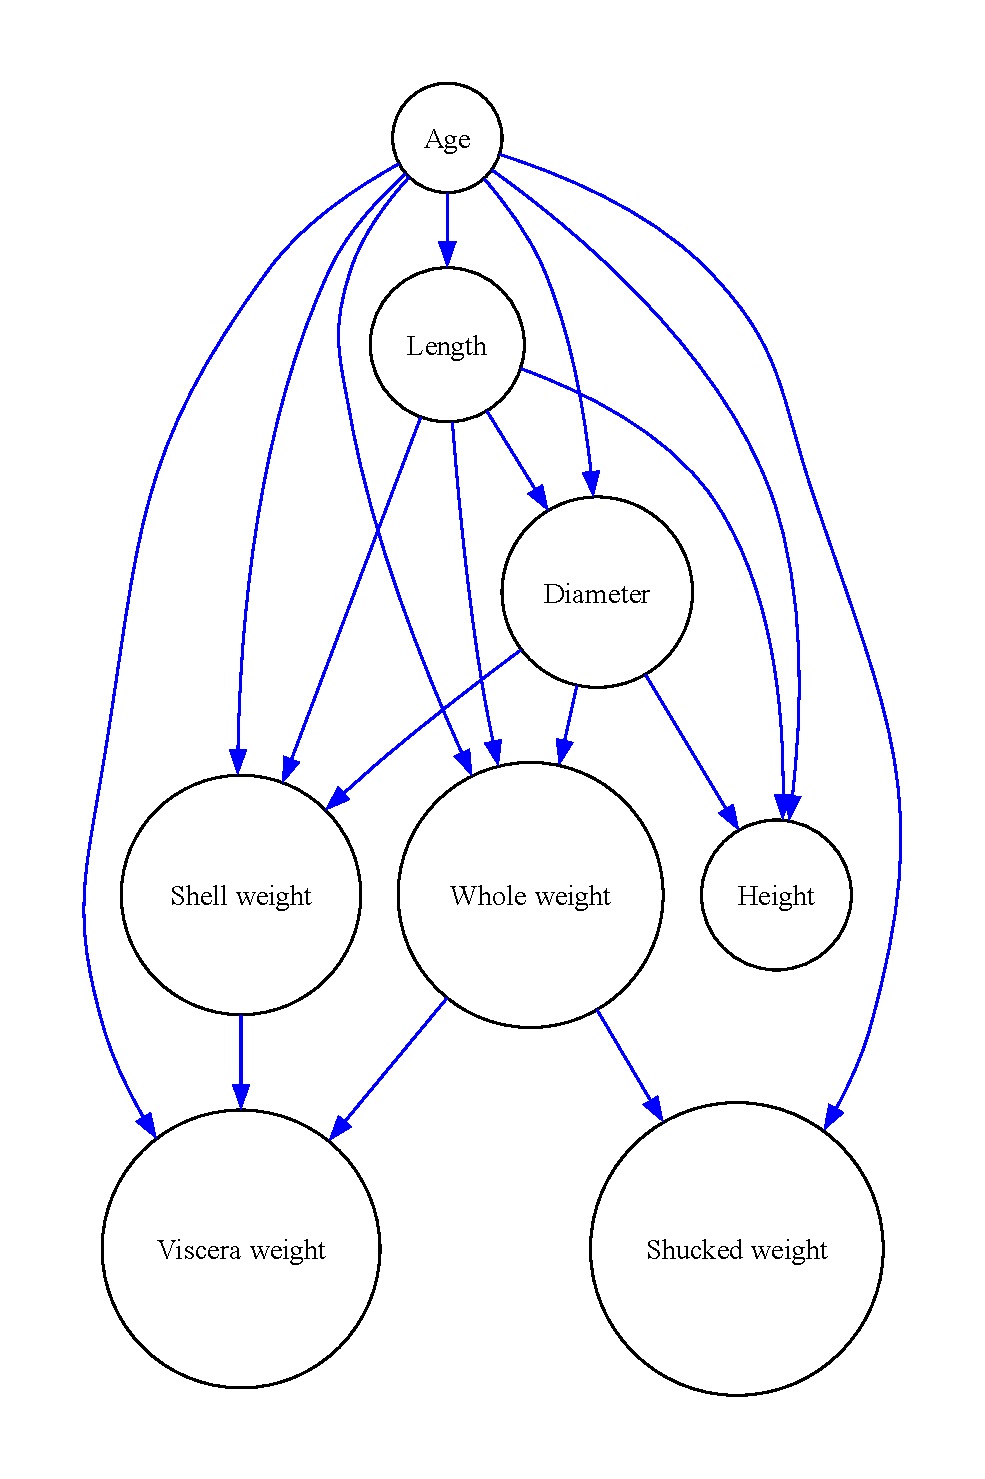
\includegraphics[height=0.4\textheight]{./demo_data/20241104_111650/Abalone/output_graph/potential_relation.pdf}}
\caption{\label{fig:relation}Possible Causal Relation Graph}
\end{figure}
\end{minipage}

\section{Dataset Descriptions and EDA}
The following is a preview of our original dataset.

\begin{table}[H]
    \centering
    \caption{Dataset Preview}
    \begin{tabular}{rrrrrrrr}
\toprule
 Age &  Length &  Shell weight &  Diameter &  Height &  Whole weight &  Shucked weight &  Viscera weight \\
\midrule
15.0 &   0.455 &         0.365 &     0.095 &  0.5140 &        0.2245 &          0.1010 &           0.150 \\
 7.0 &   0.350 &         0.265 &     0.090 &  0.2255 &        0.0995 &          0.0485 &           0.070 \\
 9.0 &   0.530 &         0.420 &     0.135 &  0.6770 &        0.2565 &          0.1415 &           0.210 \\
10.0 &   0.440 &         0.365 &     0.125 &  0.5160 &        0.2155 &          0.1140 &           0.155 \\
 7.0 &   0.330 &         0.255 &     0.080 &  0.2050 &        0.0895 &          0.0395 &           0.055 \\
\bottomrule
\end{tabular}
\end{table}

\subsection{Data Properties}
We employ several statistical methods to identify data properties.

The shape of the data, data types, and missing values are assessed directly from the dataframe.
Linearity is evaluated using Ramsey’s RESET test, followed by the Benjamini \& Yekutieli procedure for multiple test correction.
Gaussian noise is assessed through the Shapiro-Wilk test, also applying the Benjamini \& Yekutieli procedure for multiple test correction.
Time-Series and Heterogeneity are derived from user queries.

Properties of the dataset we analyzed are listed below.

\begin{table}[H]
    \centering
    \caption{Data Properties}
    \begin{tabular}{rrrrrrr}
\toprule
Shape ($n$ x $d$) & Data Type & Missing Value & Linearity & Gaussian Errors & Time-Series & Heterogeneity \\
\midrule
(4177, 8)   & Continuous & False & False & False & False & False \\
\bottomrule
\end{tabular}
\end{table}

\subsection{Distribution Analysis}
The following figure shows distributions of different variables. The orange dash line represents the mean, 
and the black line represents the median. Variables are categorized into three types according to their distribution characteristics.

\begin{figure}[H]
\centering
\includegraphics[width=\linewidth]{./demo_data/20241104_111650/Abalone/output_graph/eda_dist.jpg}
\caption{\label{fig:dist}Distribution Plots of Variables}
\end{figure}

\begin{itemize}
\item Slight left skew distributed variables: Length, Shell Weight, Diameter, Whole Weight
\item Slight right skew distributed variables: Age, Height, Shucked weight, Viscera weight
\item Symmetric distributed variables: None
\end{itemize}

\subsection{Correlation Analysis}

\begin{minipage}[t]{0.5\linewidth}
    In this analysis, we will categorize the correlation statistics of features in the dataset into three distinct categories: Strong correlations (r>0.8), Moderate correlations (0.5<r<0.8), and Weak correlations (r<0.5).

\begin{itemize}
\item Strong Correlated Variables: Shell weight and Length, Height and Whole weight, Shucked weight and Shell weight, Viscera weight and Shell weight, Viscera weight and Height
\item Moderate Correlated Variables: Length and Age, Shell weight and Age, Diameter and Age, Diameter and Length, Height and Age, Whole weight and Diameter, Shucked weight and Age, Shucked weight and Diameter, Viscera weight and Diameter, Viscera weight and Whole weight
\item Weak Correlated Variables: Shucked weight and Age
\end{itemize}
\vfill
\end{minipage}
\hfill
\begin{minipage}[t]{0.5\linewidth}
    \begin{figure}[H]
        \centering
        \vspace{-1.5cm}
        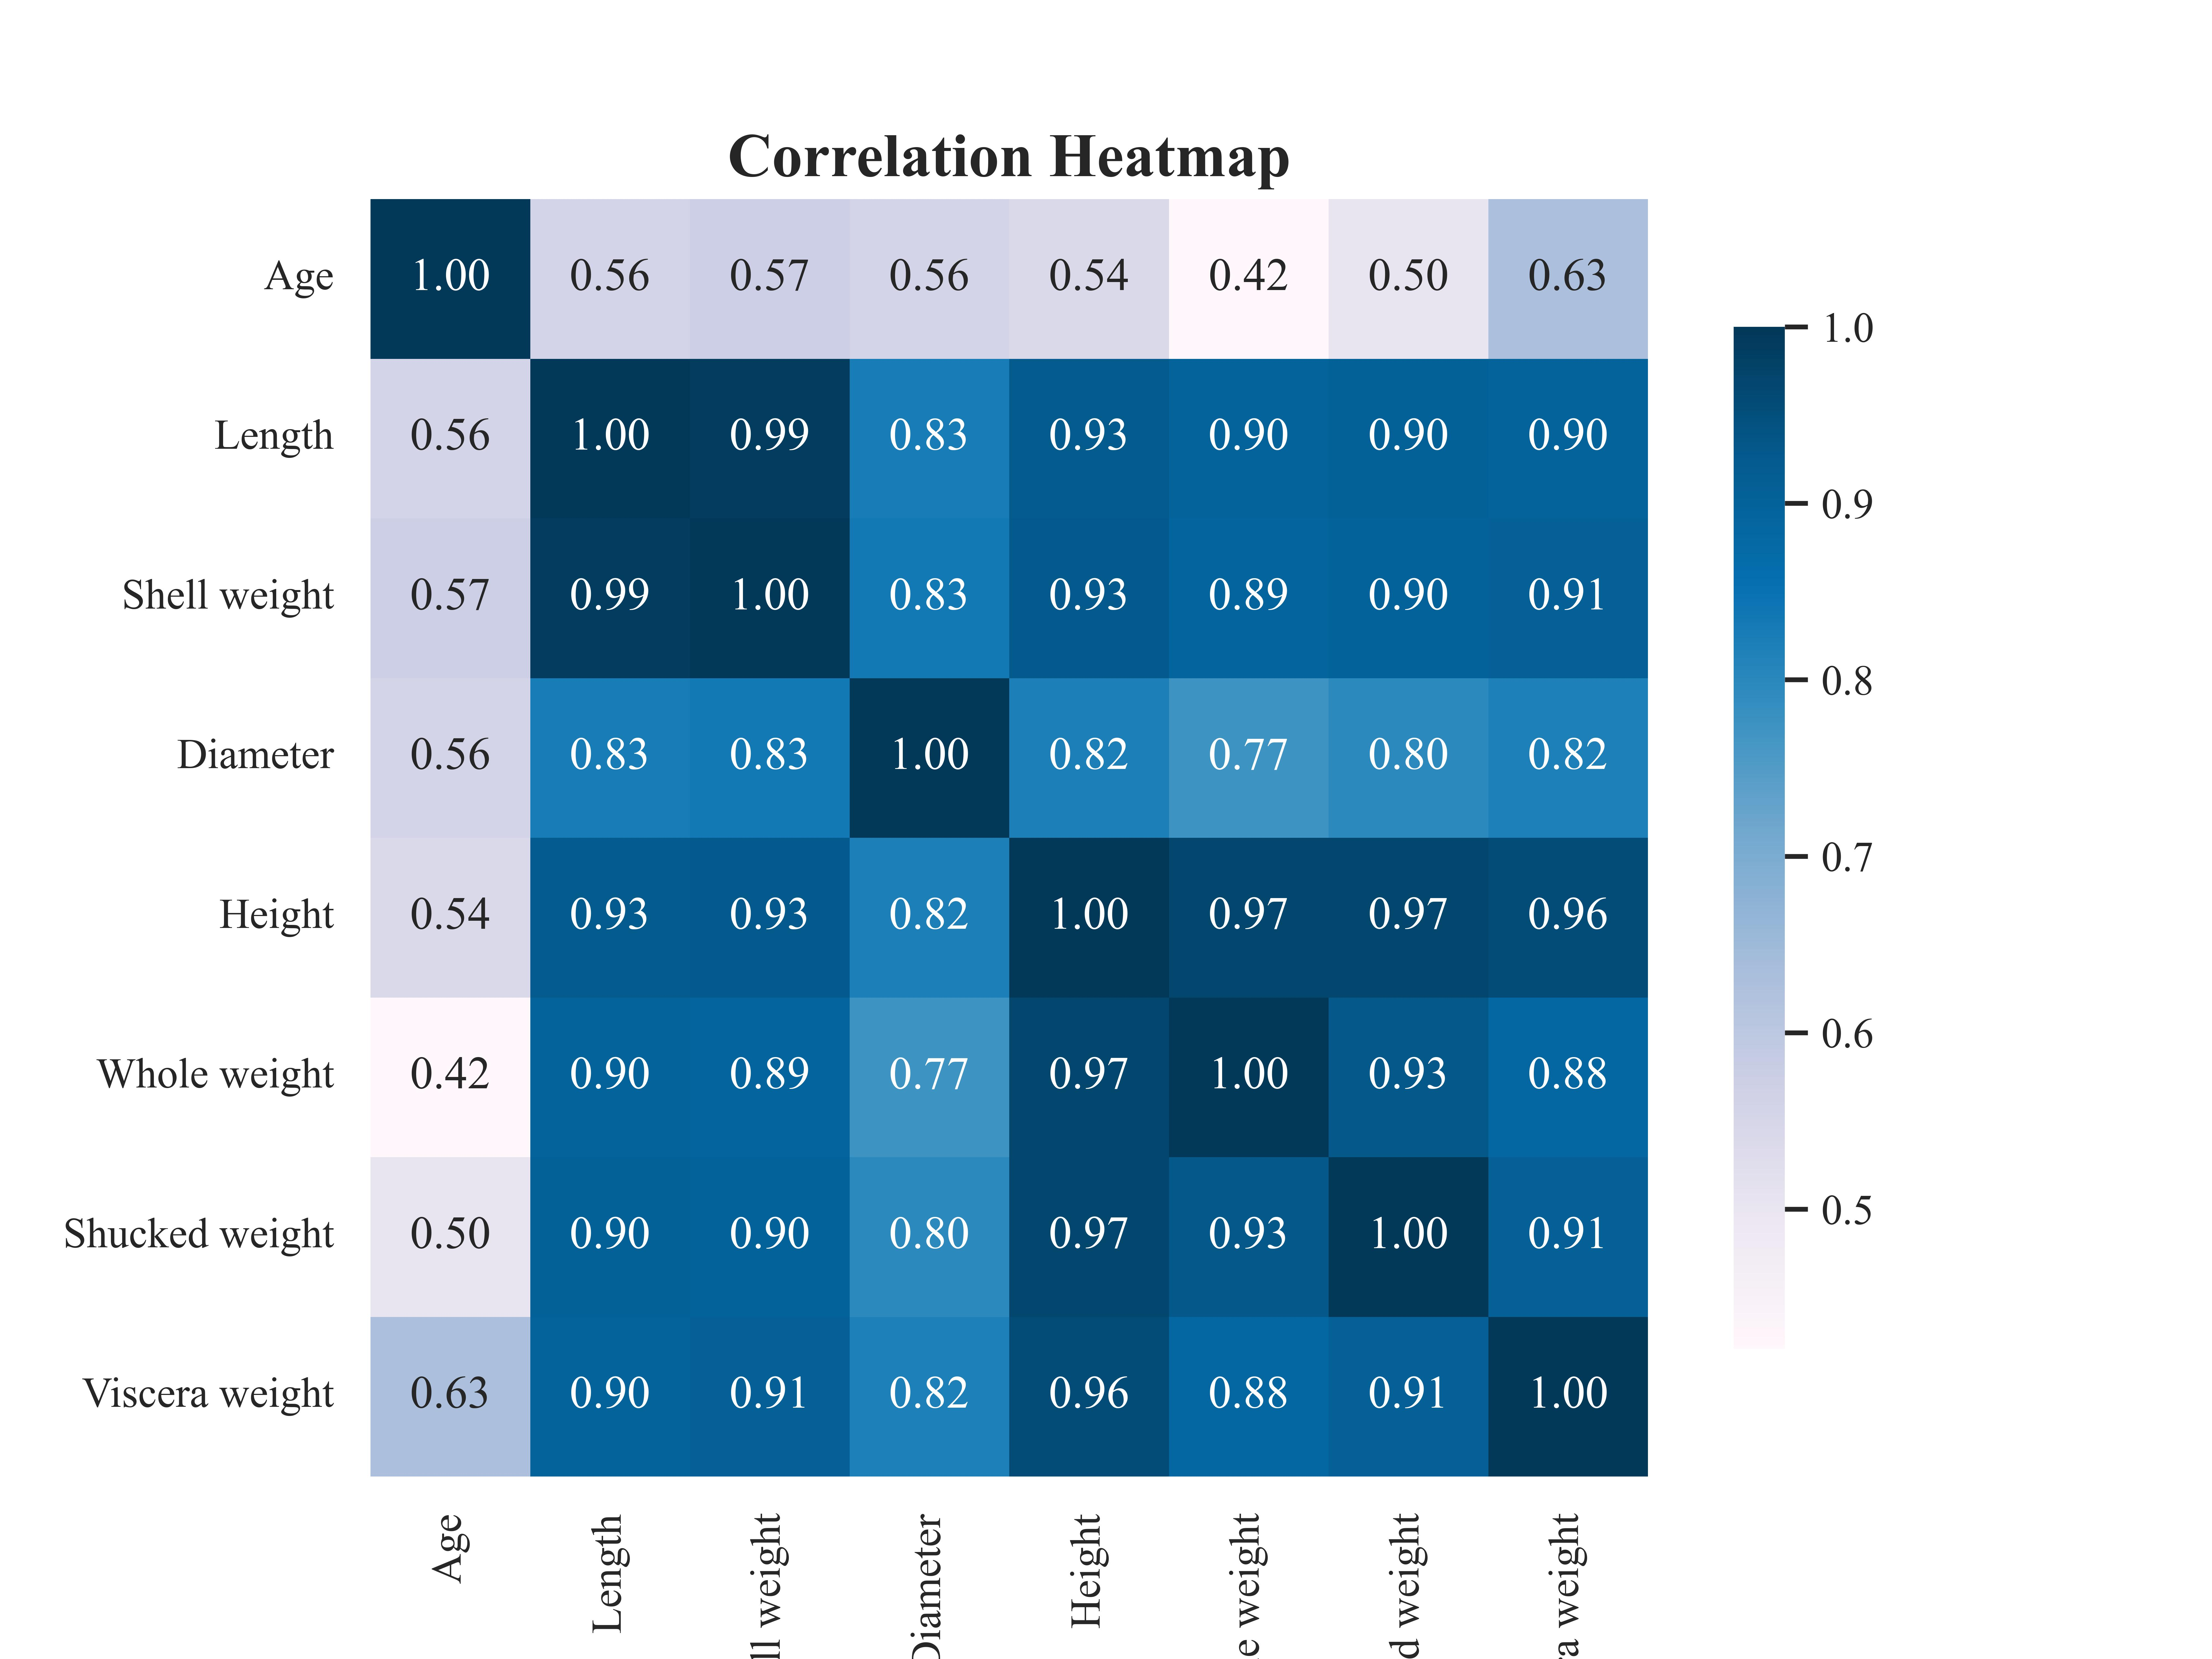
\includegraphics[width=\linewidth]{./demo_data/20241104_111650/Abalone/output_graph/eda_corr.jpg}
        \caption{\label{fig:corr}Correlation Heatmap of Variables}
    \end{figure}
\end{minipage}

\section{Discovery Procedure}
In this section, we provide a detailed description of the causal discovery process implemented by Causal Copilot. 
We also provide the chosen algorithms and hyperparameters, along with the justifications for these selections.

\subsection{Data Preprocessing}
In this initial step, we preprocessed the data and examined its statistical characteristics. 
This involved cleaning the data, handling missing values, and performing exploratory data analysis to understand distributions and relationships between variables.

\subsection{Algorithm Selection assisted with LLM}
Following data preprocessing, we employed a large language model (LLM) to assist in 
selecting appropriate algorithms for causal discovery based on the statistical characteristics of the dataset and relevant background knowledge. 
The top three chosen algorithms, listed in order of suitability, are as follows:   

\begin{itemize}
    \item \textbf{PC}:
    \begin{itemize}
        \item \textbf{Description}: The PC algorithm is a constraint-based method that learns the structure of a causal graph from data by testing conditional independencies between variables. It constructs a directed acyclic graph (DAG) representing the causal relationships.
        \item \textbf{Justification}: Given that the dataset has no missing values and a large sample size (4177), the PC algorithm is well-suited due to its efficiency in handling large datasets and its ability to discover causal relationships, assuming all relevant variables are observed.
    \end{itemize}
    
    \item \textbf{GES}:
    \begin{itemize}
        \item \textbf{Description}: Greedy Equivalence Search (GES) is a score-based causal discovery algorithm that identifies the optimal causal structure by navigating the space of equivalence classes of Directed Acyclic Graphs (DAGs).
        \item \textbf{Justification}: GES is appropriate given that it can operate effectively on large datasets and is not constrained by the linear relationships of the data, making it versatile for this dataset where linearity is not predominant.
    \end{itemize}
    
    \item \textbf{NOTEARS}:
    \begin{itemize}
        \item \textbf{Description}: NOTEARS is an algorithm that transforms the problem of learning Directed Acyclic Graphs (DAGs) into a continuous optimization problem, enabling it to efficiently scale to large datasets.
        \item \textbf{Justification}: NOTEARS is suitable for high-dimensional data and can accommodate nonlinear relationships in the dataset. It allows for efficient learning of causal structures in a continuous optimization context, making it a good candidate for such a dataset.
    \end{itemize}
    
\end{itemize}

\subsection{Hyperparameter Values Proposal assisted with LLM}
Once the algorithms were selected, the LLM aided in proposing hyperparameters 
for the chosen algorithm, which are specified below:
        
\begin{itemize}
    \item \textbf{alpha}:
    \begin{itemize}
        \item \textbf{Value}: 0.05
        \item \textbf{Explanation}: Given the sample size of 4177, which falls within the range of 500 to 10000, the default value of 0.05 is appropriate. It provides a balance between Type I error rates while being conservative enough to avoid false discoveries.
    \end{itemize}
    
    \item \textbf{indep\_test}:
    \begin{itemize}
        \item \textbf{Value}: fisherz
        \item \textbf{Explanation}: Fisher's Z test is suitable for continuous data types, which aligns with the characteristics of this dataset. Although it has assumptions about linearity and Gaussianity, it is the best choice given the absence of categorical features.
    \end{itemize}
    
    \item \textbf{depth}:
    \begin{itemize}
        \item \textbf{Value}: -1
        \item \textbf{Explanation}: For a dataset with 8 features, allowing unlimited depth (-1) is reasonable to ensure comprehensive exploration of causal relationships, as it facilitates finding all potential causal links without limiting the graph's search space.
    \end{itemize}
    
\end{itemize}

\subsection{Graph Tuning with Bootstrap and LLM Suggestion}
In the final step, we performed graph tuning with suggestions provided by the Bootstrap and LLM.
            
Firstly, we use the Bootstrap technique to get how much confidence we have on each edge in the initial graph.
If the confidence probability of a certain edge is greater than 95\% and it is not in the initial graph, we force it.
Otherwise, if the confidence probability is smaller than 5\% and it exists in the initial graph, we change it to the edge type with the highest probability.
            
After that, we utilize LLM to help us prune edges and determine the direction of undirected edges according to its knowledge repository.
In this step, LLM can use background knowledge to add some edges that are neglected by Statistical Methods.
Voting techniques are used to enhance the robustness of results given by LLM, and the results given by LLM should not change results given by Bootstrap.

By integrating insights from both Bootstrap and LLM to refine the causal graph, we can achieve improvements in graph's accuracy and robustness.

\section{Results Summary}

\subsection{Initial Graph}

\begin{figure}[H]
    \centering
    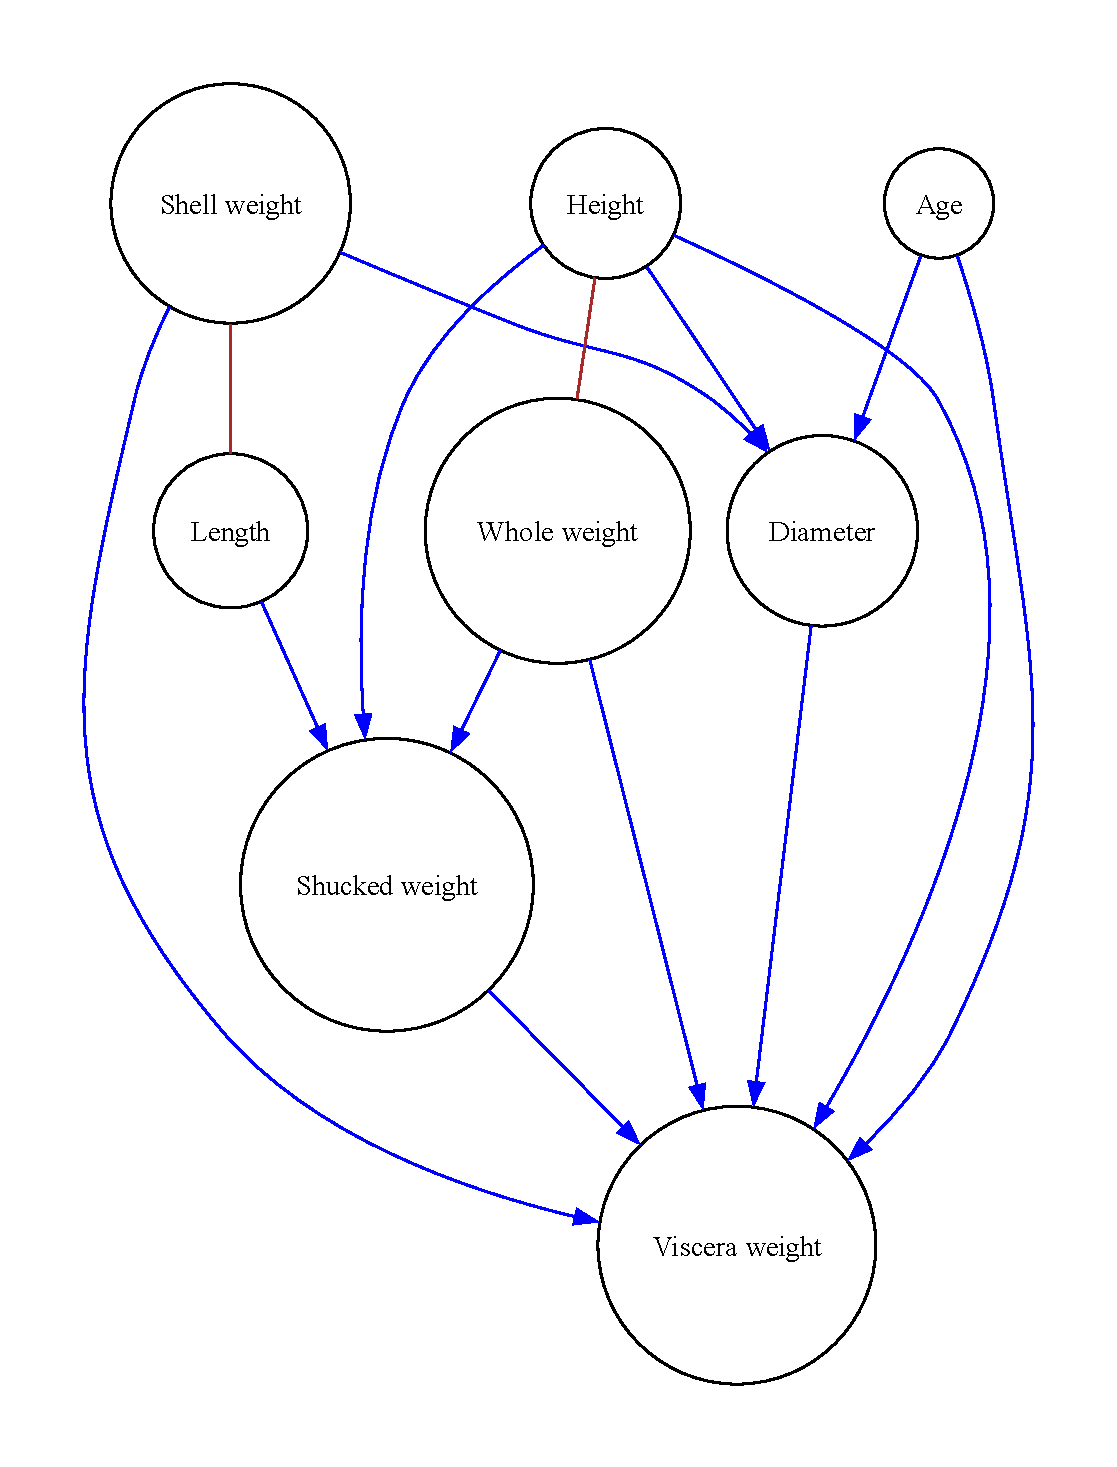
\includegraphics[width=\linewidth]{./demo_data/20241104_111650/Abalone/output_graph/initial_graph.pdf}
    \caption{Initial Graph}
\end{figure}

The above is the initial result graph produced by our algorithm.

The analysis indicates that Age has a direct influence on both Diameter and Viscera weight, suggesting that as an organism ages, its body structure and internal organs grow larger, which aligns with biological growth patterns. Length is a significant factor that affects Shell weight and Shucked weight, pointing to the idea that longer organisms tend to have greater mass and yield. Interestingly, Shell weight also influences Diameter and Viscera weight, reinforcing the notion that more substantial shells correlate with larger body sizes and greater internal mass. Furthermore, Height contributes to changes in Diameter, Whole weight, Shucked weight, and Viscera weight, indicating that taller organisms are likely to possess increased dimensions and overall mass. Whole weight, interlinked with Height and Shucked weight, reflects the comprehensive biomass of the organism and its dependence on both size and structure. Lastly, Shucked weight affects Viscera weight, demonstrating that the processing of the organism's meat is also associated with its overall internal weight, thereby highlighting the interconnected nature of these variables and their significance in understanding organism growth and development.

\subsection{Revised Graph}

\begin{minipage}[t]{0.6\linewidth}
By using the method mentioned in Section 4.4, we provide a revised graph pruned with Bootstrap and LLM suggestion.
Pruning results are as follows.
        
            Bootstrap doesn't force or forbid any edges.
            
            The following are force results given by LLM:
            
            \begin{itemize}
                \item \textbf{Age $\rightarrow$ Length}: As abalones age, they generally grow larger, resulting in an increase in shell Length, making Age a causal factor for Length.
                
                \item \textbf{Age $\rightarrow$ Shell weight}: Older abalones typically develop heavier shells due to increased size and maturity, thus Age contributes to Shell Weight.
                
                \item \textbf{Age $\rightarrow$ Height}: With age, abalones grow in height as part of their overall shell development, indicating that Age influences Height.
                
                \item \textbf{Age $\rightarrow$ Whole weight}: The overall size and health of an abalone increase with age, which directly affects its Whole Weight, establishing a causal relationship.
                
                \item \textbf{Age $\rightarrow$ Shucked weight}: As abalones age and grow larger, the amount of meat they carry (Shucked Weight) increases, indicating Age affects Shucked Weight.
                
                \item \textbf{Length $\rightarrow$ Diameter}: Increases in Length typically correlate with increases in Diameter, as these two dimensions represent different aspects of the same growth process.
                
                \item \textbf{Length $\rightarrow$ Height}: A larger Length often leads to a proportional increase in Height, reflecting the overall development of the abalone's shell.
                
                \item \textbf{Length $\rightarrow$ Whole weight}: Greater Length usually implies a larger and heavier abalone, thus Length is a causal factor for Whole Weight.
                
                \item \textbf{Length $\rightarrow$ Viscera weight}: As the Length of an abalone increases, it often also means more body volume, leading to an increase in Viscera Weight.
                
                \item \textbf{Height $\rightarrow$ Shell weight}: A taller shell (Height) is often thicker and hence heavier, establishing a causal relationship between Height and Shell Weight.
                
            \end{itemize}
            
The following are directions of remaining undirected edges determined by the LLM:
            \begin{itemize}
            \item \textbf{Length $\rightarrow$ Shell weight}: As the length of the abalone increases with age and overall health, it is expected that the shell weight will also increase. A larger shell indicates that the abalone has had sufficient nutrition and time to grow, contributing to heavier shell weight.

            \item \textbf{Height $\rightarrow$ Whole weight}: The height of the abalone is likely to correlate positively with its whole weight, as a taller and more developed shell generally supports more body mass, reflecting better overall health and growth condition.
            \end{itemize}
            
This structured approach ensures a comprehensive and methodical analysis of the causal relationships within the dataset.
        
\vfill
\end{minipage}
\hfill
\begin{minipage}[t]{0.4\linewidth}
    \begin{figure}[H]
        \centering
        \vspace{-0.5cm}
        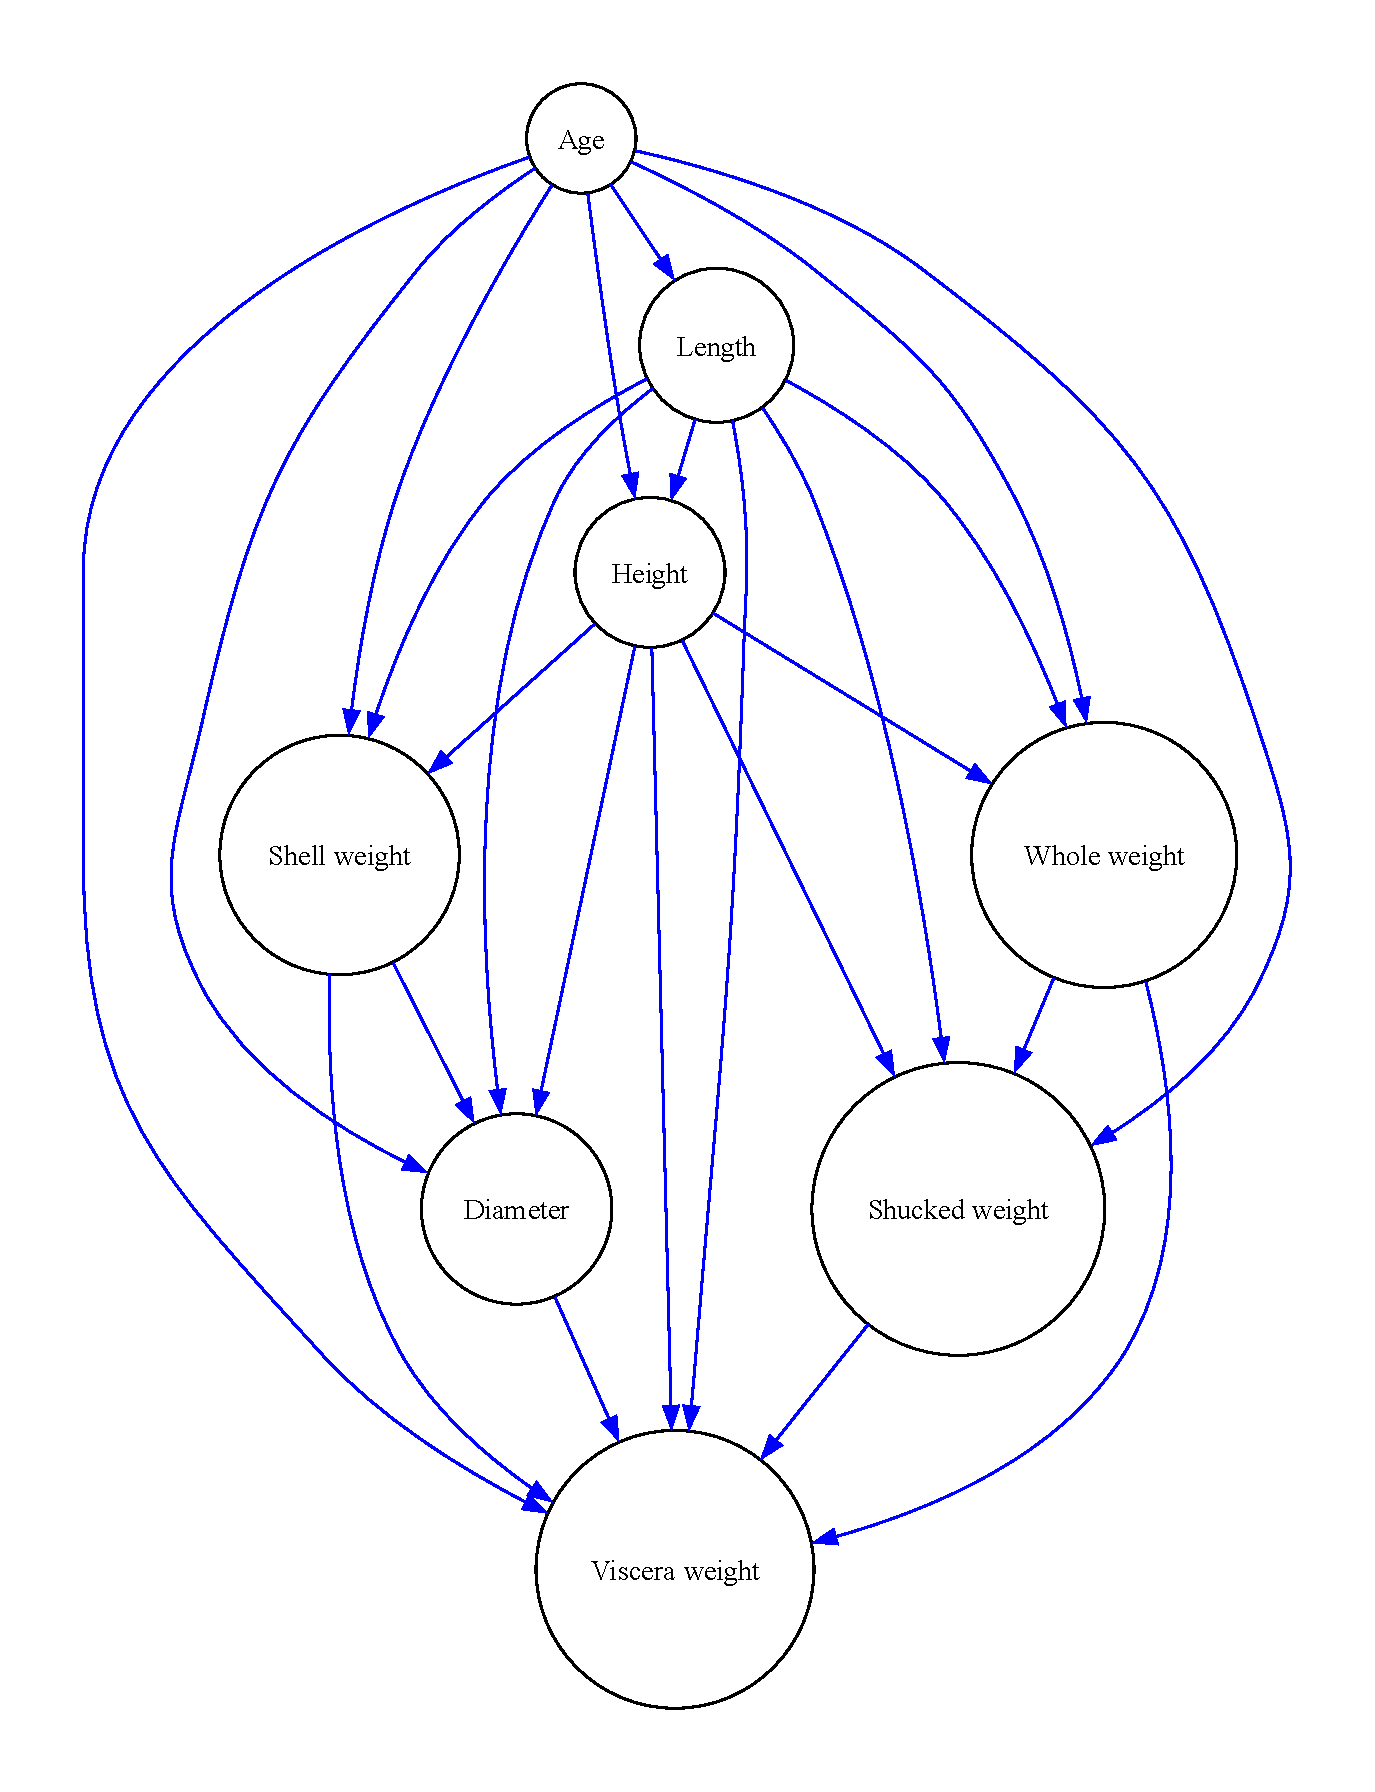
\includegraphics[width=\linewidth]{./demo_data/20241104_111650/Abalone/output_graph/revised_graph.pdf}
        \caption{\label{fig:corr}Revised Graph}
    \end{figure}
\end{minipage}

\subsection{Graph Reliability Analysis}

\begin{figure}[H]
    \centering
    \begin{subfigure}{0.32\textwidth}
        \centering
        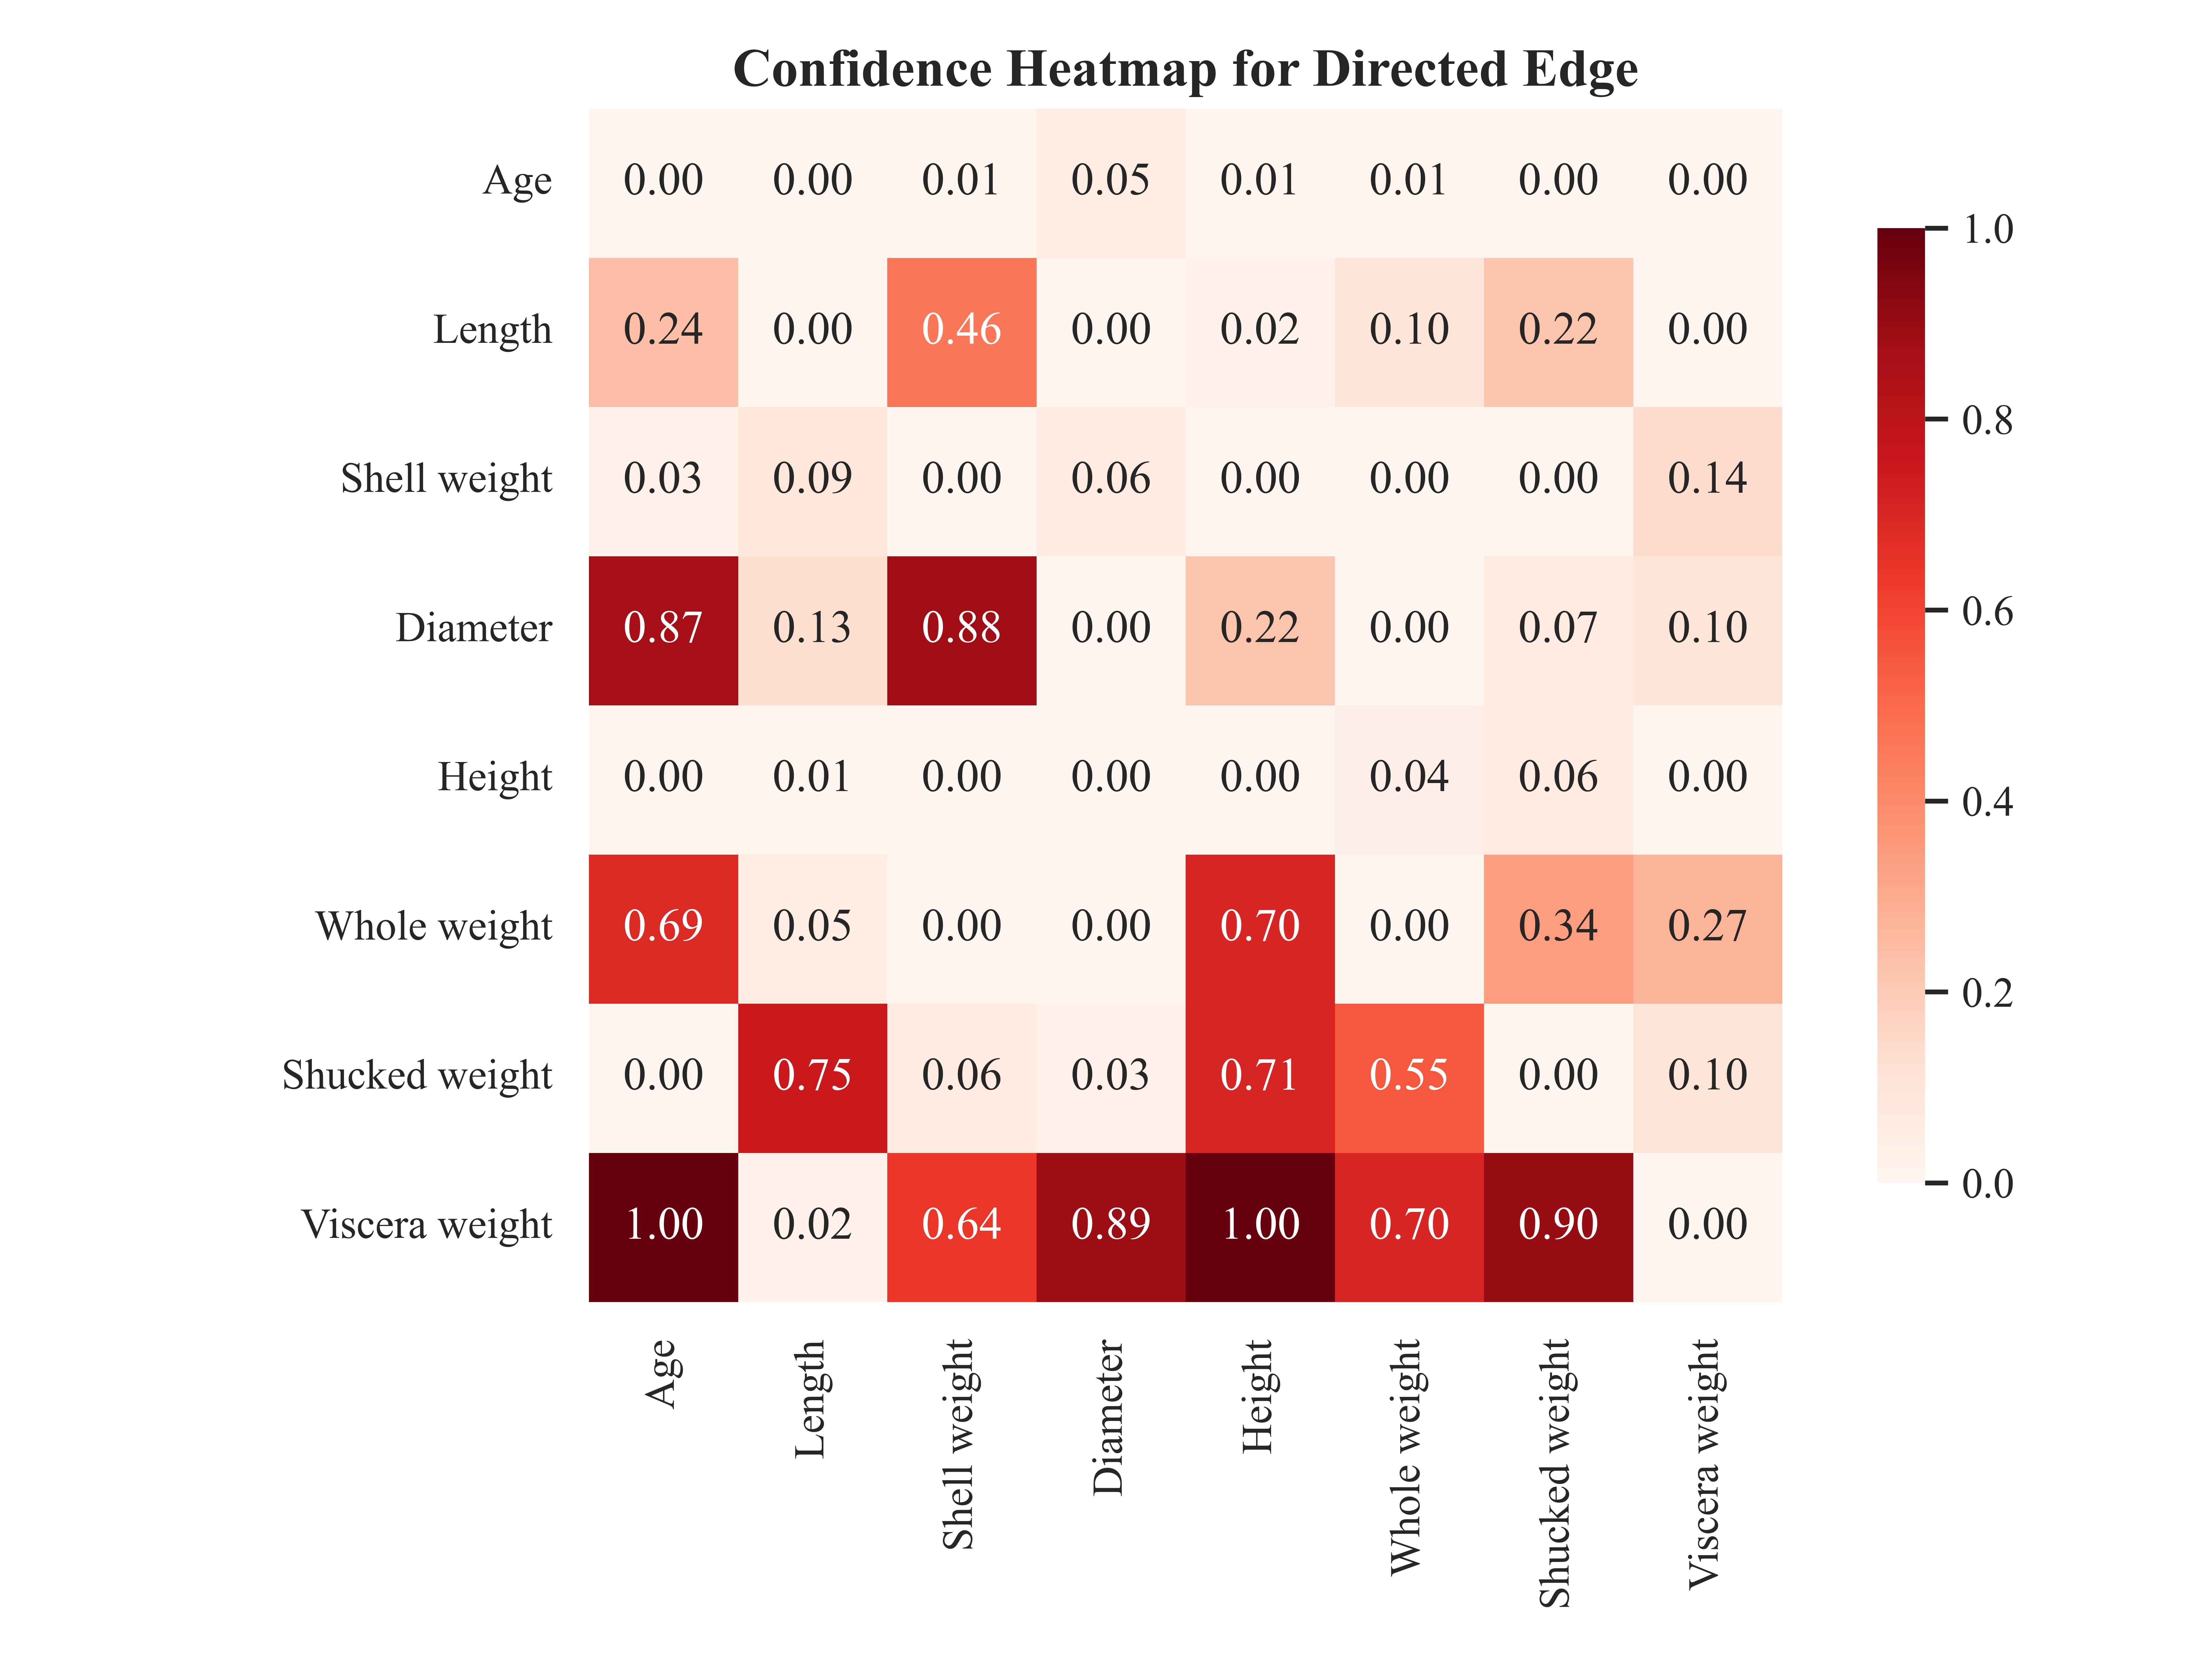
\includegraphics[width=\linewidth]{./demo_data/20241104_111650/Abalone/output_graph/certain_edges_confidence_heatmap.jpg}
        \caption{Directed Edge}
    \end{subfigure}
    \begin{subfigure}{0.32\textwidth}
        \centering
        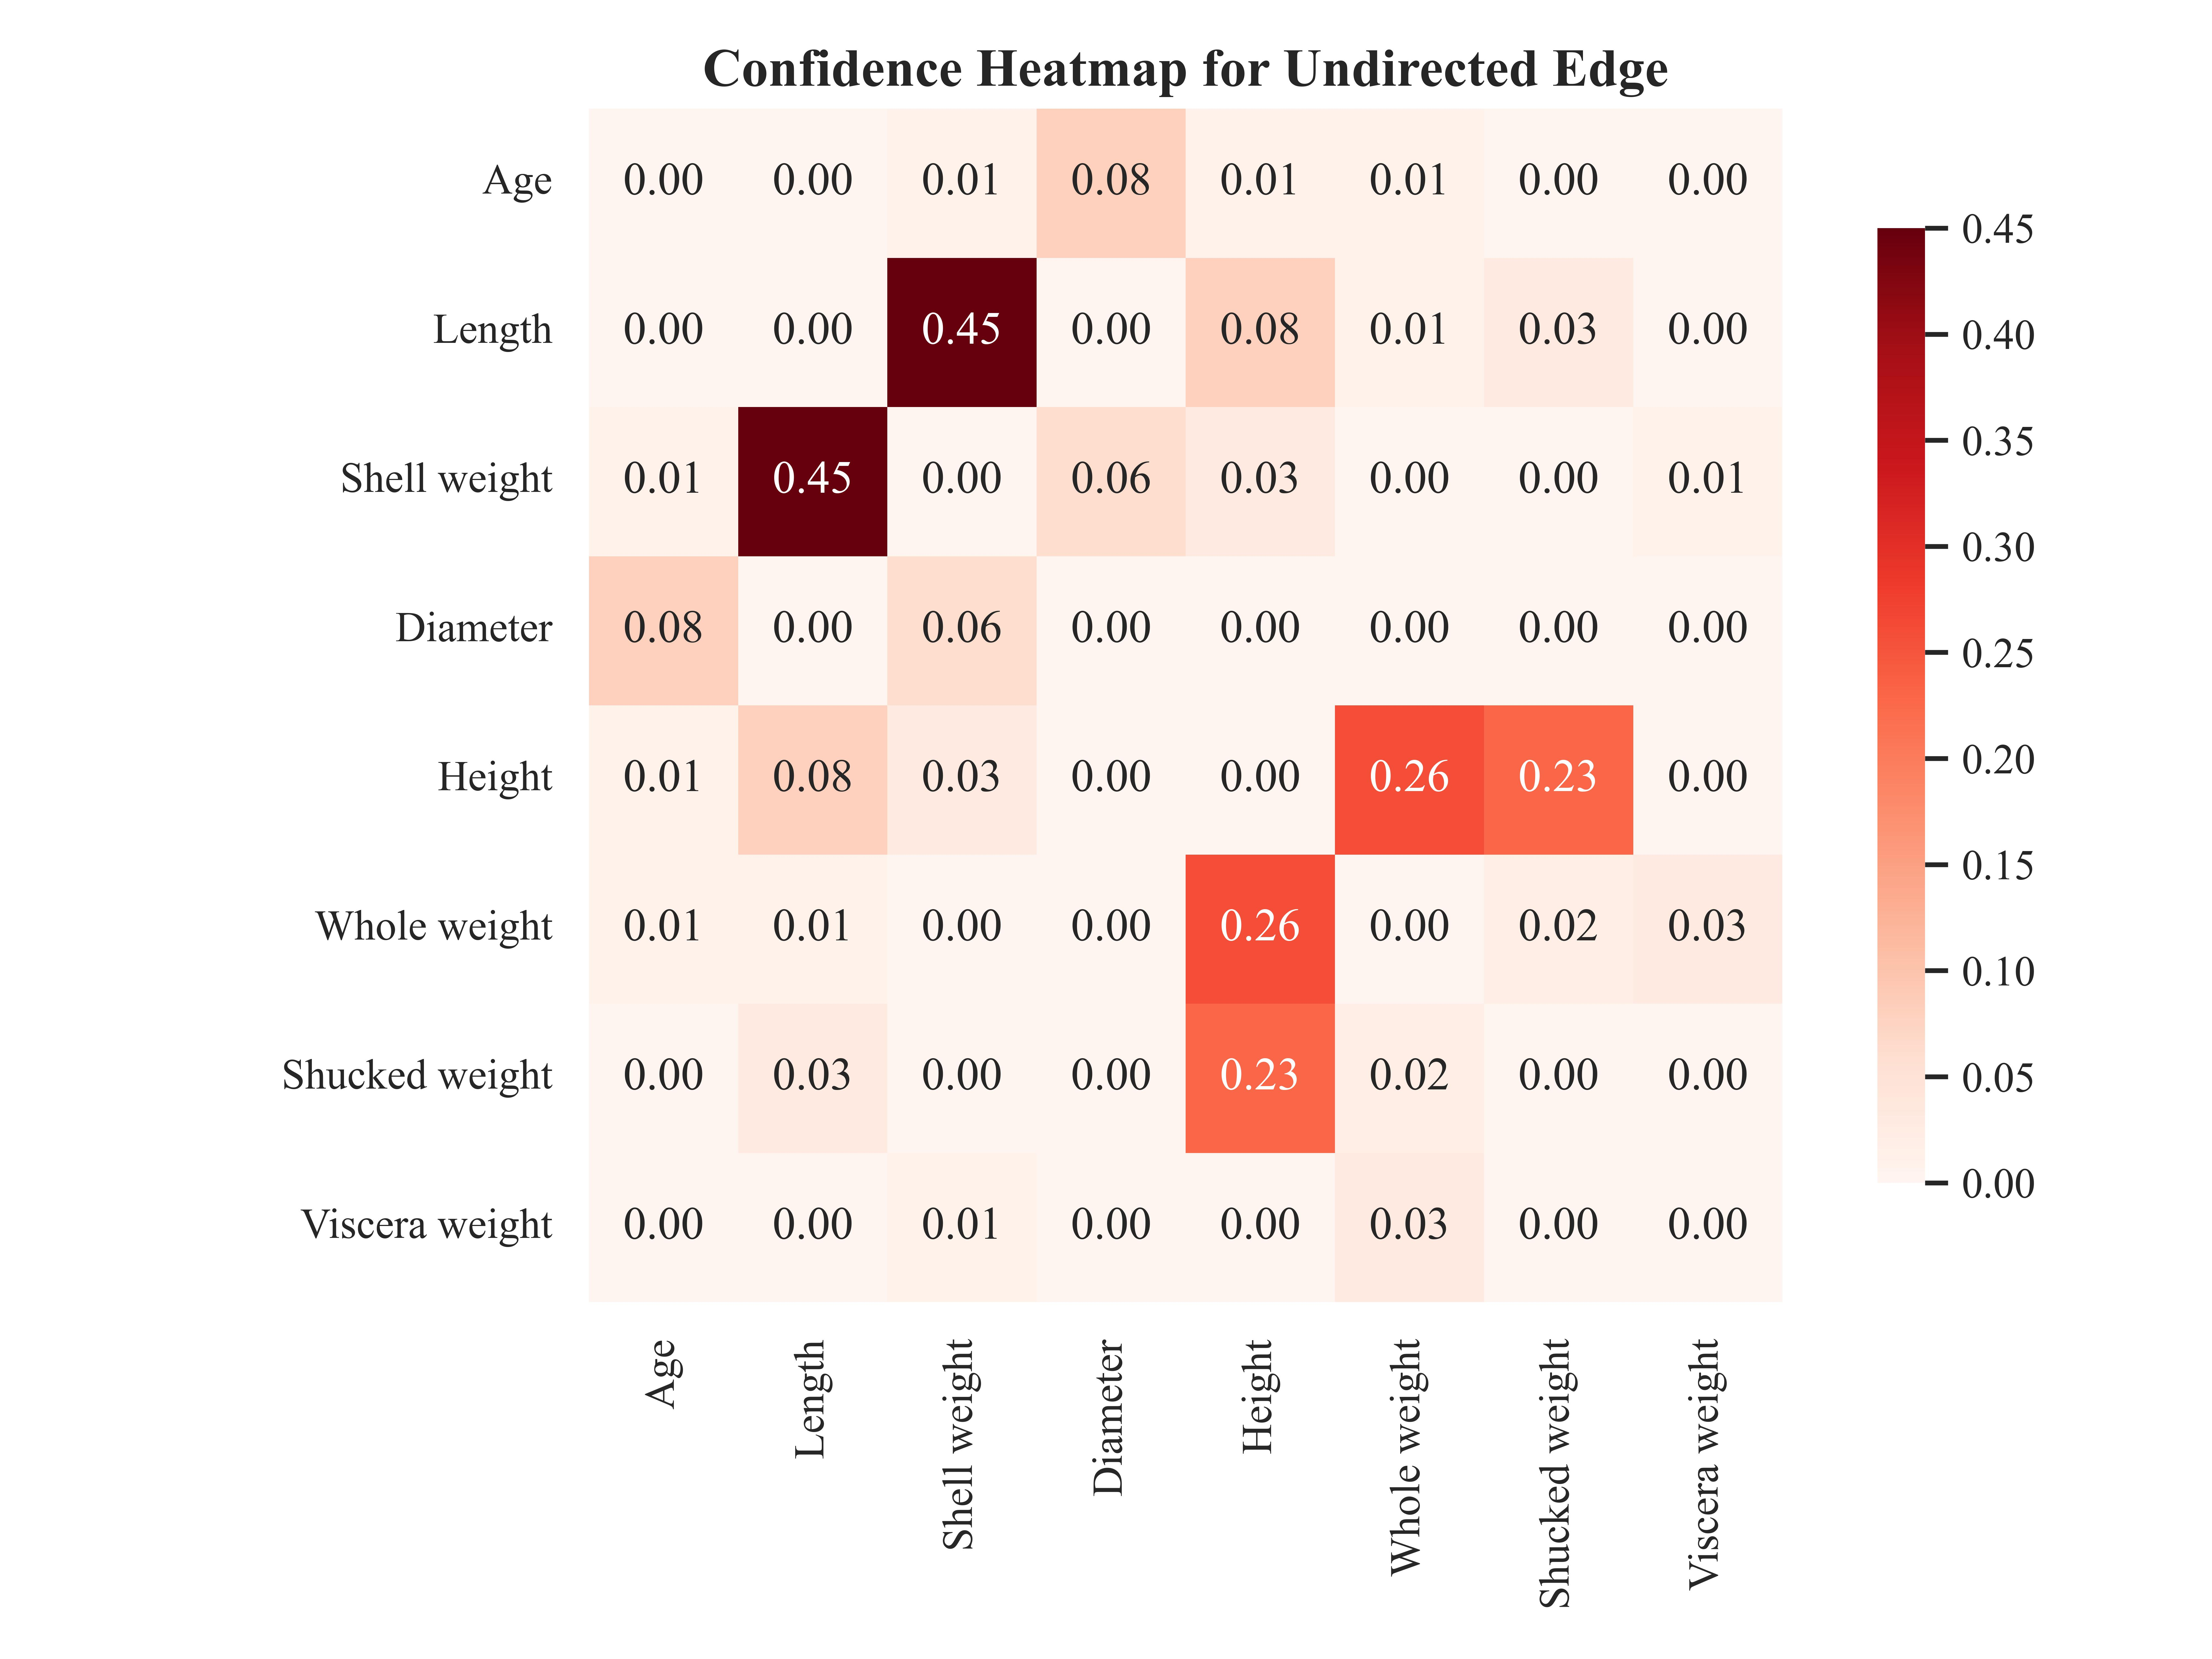
\includegraphics[width=\linewidth]{./demo_data/20241104_111650/Abalone/output_graph/uncertain_edges_confidence_heatmap.jpg}
        \caption{Undirected Edge}
    \end{subfigure}
    \begin{subfigure}{0.32\textwidth}
        \centering
        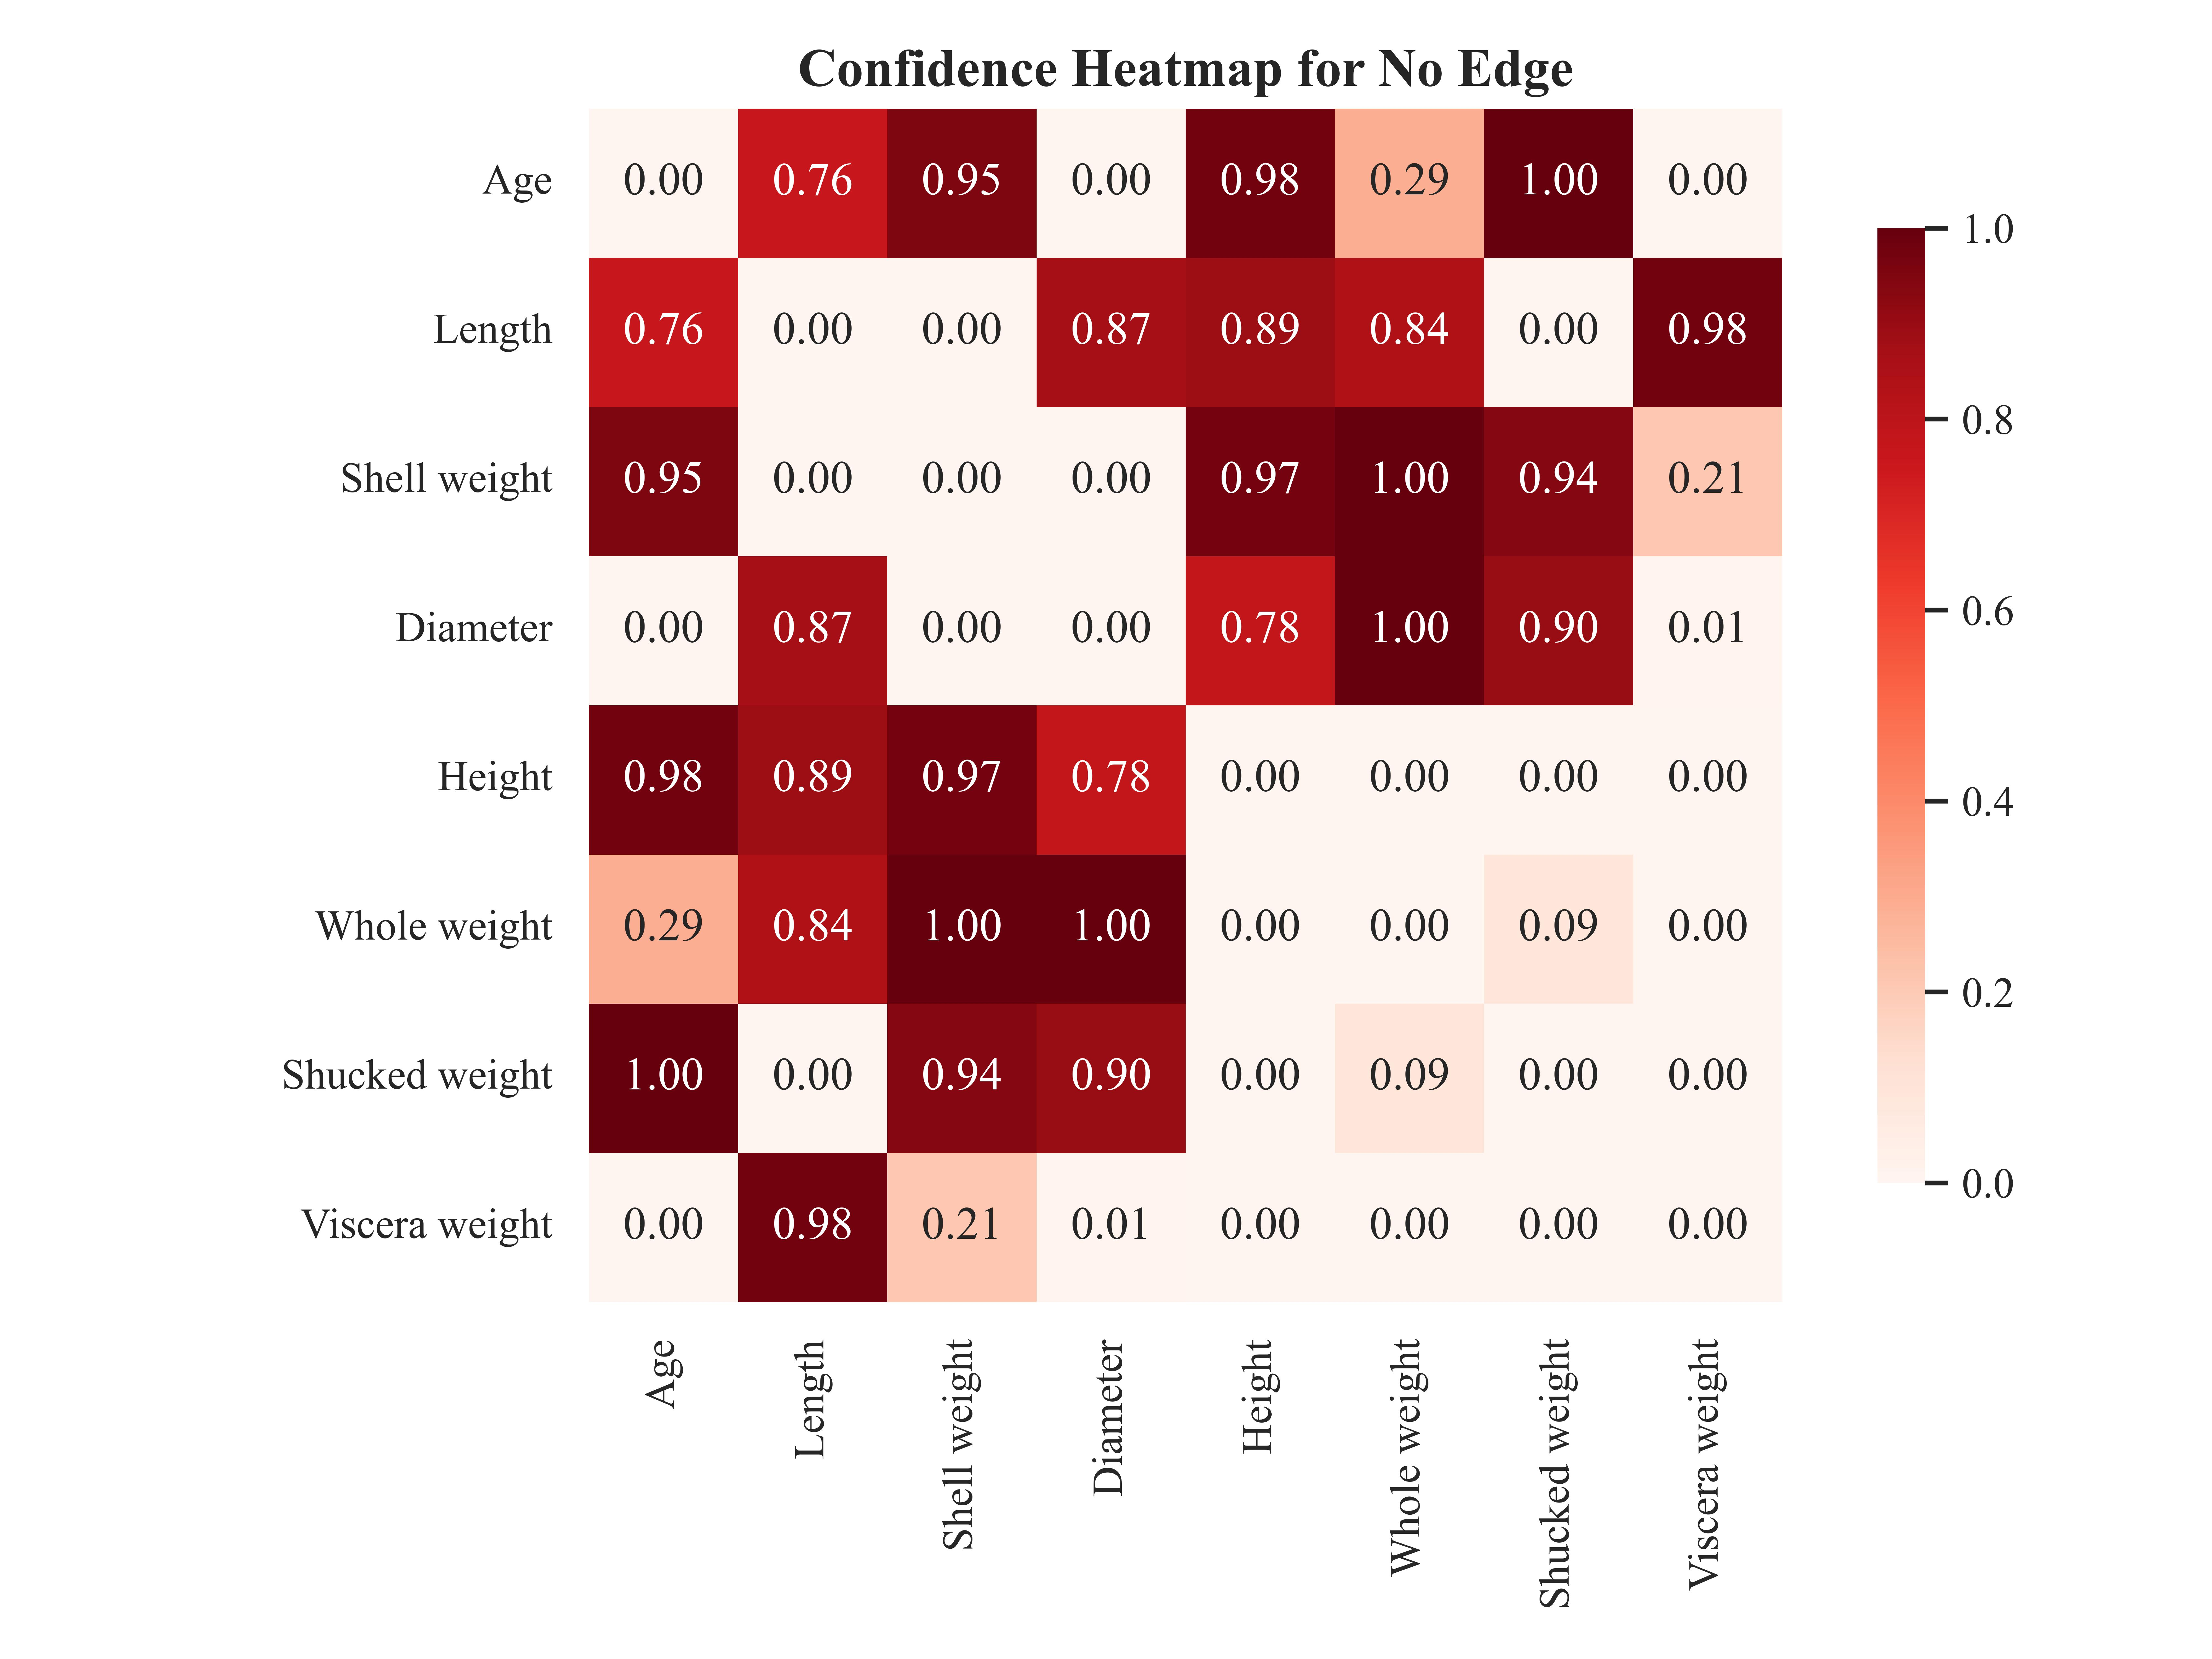
\includegraphics[width=\linewidth]{./demo_data/20241104_111650/Abalone/output_graph/non_existence_confidence_heatmap.jpg}
        \caption{No Edge}
    \end{subfigure}
    \caption{Confidence Heatmap of Different Edges}
\end{figure}        
The above heatmaps show the confidence probability we have on different kinds of edges, including directed edge ($\rightarrow$), undirected edge ($-$), No Edge, and probability of no edge. The heatmap of bi-edges is not shown because probabilities of all edges are 0. Based on the confidence probability heatmap and background knowledge, we can analyze the reliability of our graph.

From the statistics perspective, we have high confidence to believe that the following edges exist due to bootstrap probabilities: Whole weight $\rightarrow$ Height (0.7), Whole weight $\rightarrow$ Shucked weight (0.34), and Length $\rightarrow$ Shell weight (0.46). On the other hand, we have low confidence in the existence of the edges Age $\rightarrow$ Viscera weight (0.0), Height $\rightarrow$ Diameter (0.0), and Age $\rightarrow$ Diameter (0.05). These low probabilities indicate uncertainty about these causal relationships.

However, based on expert knowledge, we know that several of these edges are indeed plausible causative relationships. For example, Age is likely to influence all other size-related variables (Length, Diameter, Height), as older abalones typically grow larger. While the statistical evidence suggests a weak link between Age and Diameter, expert biological understanding supports the idea of a causal relationship. Conversely, the edges relating to Shucked weight and Whole weight are well-supported by both statistical probability and domain knowledge due to their intrinsic link in the biological context.

Therefore, while there is some statistical uncertainty regarding specific edges, the strong alignment of expert knowledge with the causal relationships involving age, size, and weight metrics suggests that this causal graph is reliable overall. However, caution should be taken regarding edges with low bootstrap probabilities, particularly those that diverge from established biological correlations.

\end{document}